\documentclass[1p]{elsarticle_modified}
%\bibliographystyle{elsarticle-num}

%\usepackage[colorlinks]{hyperref}
%\usepackage{abbrmath_seonhwa} %\Abb, \Ascr, \Acal ,\Abf, \Afrak
\usepackage{amsfonts}
\usepackage{amssymb}
\usepackage{amsmath}
\usepackage{amsthm}
\usepackage{scalefnt}
\usepackage{amsbsy}
\usepackage{kotex}
\usepackage{caption}
\usepackage{subfig}
\usepackage{color}
\usepackage{graphicx}
\usepackage{xcolor} %% white, black, red, green, blue, cyan, magenta, yellow
\usepackage{float}
\usepackage{setspace}
\usepackage{hyperref}

\usepackage{tikz}
\usetikzlibrary{arrows}

\usepackage{multirow}
\usepackage{array} % fixed length table
\usepackage{hhline}

%%%%%%%%%%%%%%%%%%%%%
\makeatletter
\renewcommand*\env@matrix[1][\arraystretch]{%
	\edef\arraystretch{#1}%
	\hskip -\arraycolsep
	\let\@ifnextchar\new@ifnextchar
	\array{*\c@MaxMatrixCols c}}
\makeatother %https://tex.stackexchange.com/questions/14071/how-can-i-increase-the-line-spacing-in-a-matrix
%%%%%%%%%%%%%%%

\usepackage[normalem]{ulem}

\newcommand{\msout}[1]{\ifmmode\text{\sout{\ensuremath{#1}}}\else\sout{#1}\fi}
%SOURCE: \msout is \stkout macro in https://tex.stackexchange.com/questions/20609/strikeout-in-math-mode

\newcommand{\cancel}[1]{
	\ifmmode
	{\color{red}\msout{#1}}
	\else
	{\color{red}\sout{#1}}
	\fi
}

\newcommand{\add}[1]{
	{\color{blue}\uwave{#1}}
}

\newcommand{\replace}[2]{
	\ifmmode
	{\color{red}\msout{#1}}{\color{blue}\uwave{#2}}
	\else
	{\color{red}\sout{#1}}{\color{blue}\uwave{#2}}
	\fi
}

\newcommand{\Sol}{\mathcal{S}} %segment
\newcommand{\D}{D} %diagram
\newcommand{\A}{\mathcal{A}} %arc


%%%%%%%%%%%%%%%%%%%%%%%%%%%%%5 test

\def\sl{\operatorname{\textup{SL}}(2,\Cbb)}
\def\psl{\operatorname{\textup{PSL}}(2,\Cbb)}
\def\quan{\mkern 1mu \triangleright \mkern 1mu}

\theoremstyle{definition}
\newtheorem{thm}{Theorem}[section]
\newtheorem{prop}[thm]{Proposition}
\newtheorem{lem}[thm]{Lemma}
\newtheorem{ques}[thm]{Question}
\newtheorem{cor}[thm]{Corollary}
\newtheorem{defn}[thm]{Definition}
\newtheorem{exam}[thm]{Example}
\newtheorem{rmk}[thm]{Remark}
\newtheorem{alg}[thm]{Algorithm}

\newcommand{\I}{\sqrt{-1}}
\begin{document}

%\begin{frontmatter}
%
%\title{Boundary parabolic representations of knots up to 8 crossings}
%
%%% Group authors per affiliation:
%\author{Yunhi Cho} 
%\address{Department of Mathematics, University of Seoul, Seoul, Korea}
%\ead{yhcho@uos.ac.kr}
%
%
%\author{Seonhwa Kim} %\fnref{s_kim}}
%\address{Center for Geometry and Physics, Institute for Basic Science, Pohang, 37673, Korea}
%\ead{ryeona17@ibs.re.kr}
%
%\author{Hyuk Kim}
%\address{Department of Mathematical Sciences, Seoul National University, Seoul 08826, Korea}
%\ead{hyukkim@snu.ac.kr}
%
%\author{Seokbeom Yoon}
%\address{Department of Mathematical Sciences, Seoul National University, Seoul, 08826,  Korea}
%\ead{sbyoon15@snu.ac.kr}
%
%\begin{abstract}
%We find all boundary parabolic representation of knots up to 8 crossings.
%
%\end{abstract}
%\begin{keyword}
%    \MSC[2010] 57M25 
%\end{keyword}
%
%\end{frontmatter}

%\linenumbers
%\tableofcontents
%
\newcommand\colored[1]{\textcolor{white}{\rule[-0.35ex]{0.8em}{1.4ex}}\kern-0.8em\color{red} #1}%
%\newcommand\colored[1]{\textcolor{white}{ #1}\kern-2.17ex	\textcolor{white}{ #1}\kern-1.81ex	\textcolor{white}{ #1}\kern-2.15ex\color{red}#1	}

{\Large $\underline{10_{151}~(K10n_{8})}$}

\setlength{\tabcolsep}{10pt}
\renewcommand{\arraystretch}{1.6}
\vspace{1cm}\begin{tabular}{m{100pt}>{\centering\arraybackslash}m{274pt}}
\multirow{5}{120pt}{
	\centering
	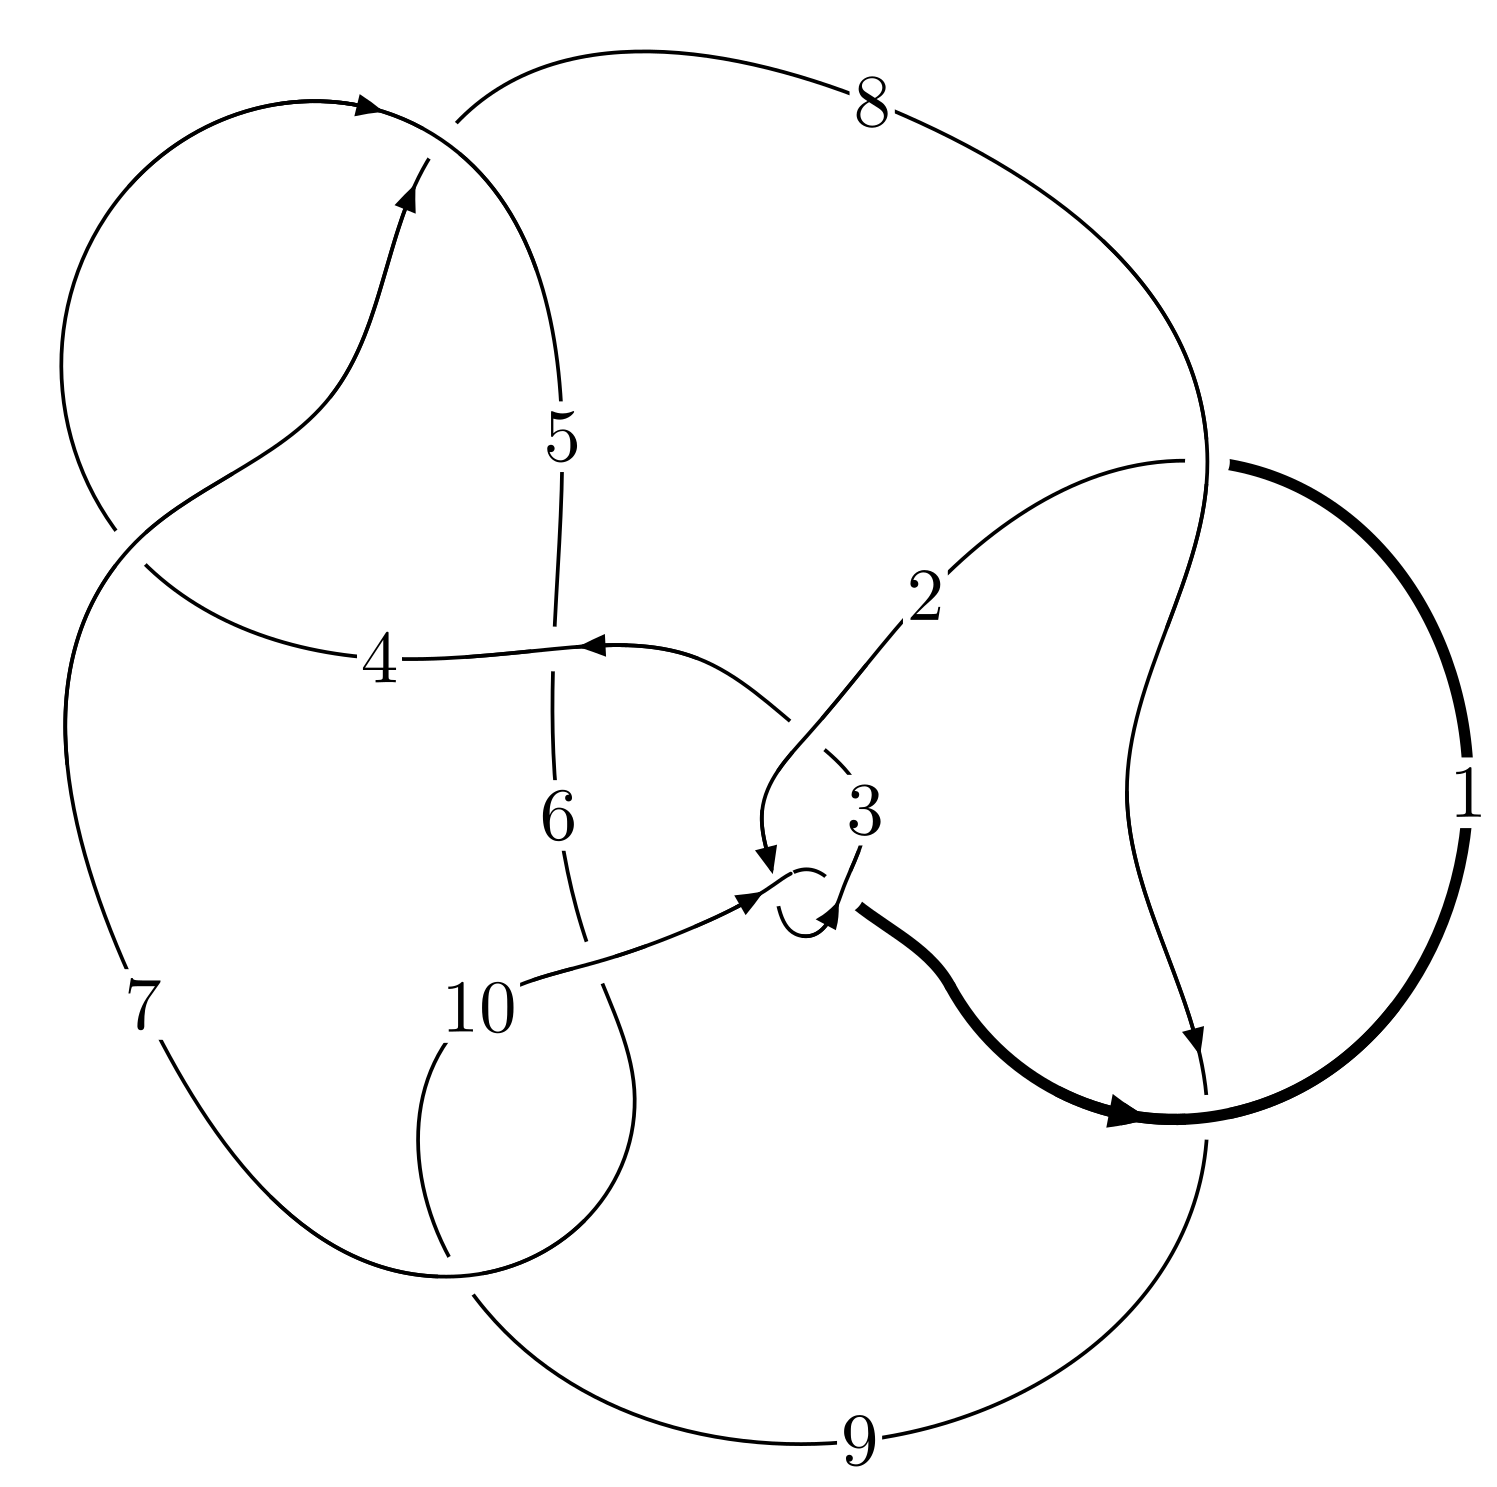
\includegraphics[width=112pt]{../../../GIT/diagram.site/Diagrams/png/235_10_151.png}\\
\ \ \ A knot diagram\footnotemark}&
\allowdisplaybreaks
\textbf{Linearized knot diagam} \\
\cline{2-2}
 &
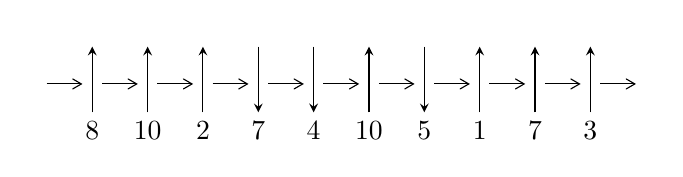
\begin{tikzpicture}[x=20pt, y=17pt]
	% nodes
	\node (C0) at (0, 0) {};
	\node (C1) at (1, 0) {};
	\node (C1U) at (1, +1) {};
	\node (C1D) at (1, -1) {8};

	\node (C2) at (2, 0) {};
	\node (C2U) at (2, +1) {};
	\node (C2D) at (2, -1) {10};

	\node (C3) at (3, 0) {};
	\node (C3U) at (3, +1) {};
	\node (C3D) at (3, -1) {2};

	\node (C4) at (4, 0) {};
	\node (C4U) at (4, +1) {};
	\node (C4D) at (4, -1) {7};

	\node (C5) at (5, 0) {};
	\node (C5U) at (5, +1) {};
	\node (C5D) at (5, -1) {4};

	\node (C6) at (6, 0) {};
	\node (C6U) at (6, +1) {};
	\node (C6D) at (6, -1) {10};

	\node (C7) at (7, 0) {};
	\node (C7U) at (7, +1) {};
	\node (C7D) at (7, -1) {5};

	\node (C8) at (8, 0) {};
	\node (C8U) at (8, +1) {};
	\node (C8D) at (8, -1) {1};

	\node (C9) at (9, 0) {};
	\node (C9U) at (9, +1) {};
	\node (C9D) at (9, -1) {7};

	\node (C10) at (10, 0) {};
	\node (C10U) at (10, +1) {};
	\node (C10D) at (10, -1) {3};
	\node (C11) at (11, 0) {};

	% arrows
	\draw[->,>={angle 60}]
	(C0) edge (C1) (C1) edge (C2) (C2) edge (C3) (C3) edge (C4) (C4) edge (C5) (C5) edge (C6) (C6) edge (C7) (C7) edge (C8) (C8) edge (C9) (C9) edge (C10) (C10) edge (C11) ;	\draw[->,>=stealth]
	(C1D) edge (C1U) (C2D) edge (C2U) (C3D) edge (C3U) (C4U) edge (C4D) (C5U) edge (C5D) (C6D) edge (C6U) (C7U) edge (C7D) (C8D) edge (C8U) (C9D) edge (C9U) (C10D) edge (C10U) ;
	\end{tikzpicture} \\
\hhline{~~} \\& 
\textbf{Solving Sequence} \\ \cline{2-2} 
 &
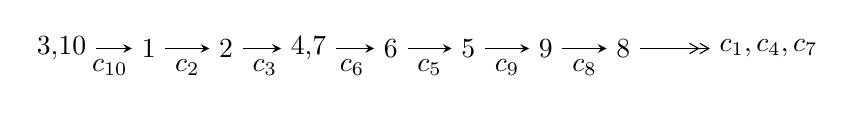
\begin{tikzpicture}[x=28pt, y=7pt]
	% node
	\node (A0) at (-1/8, 0) {3,10};
	\node (A1) at (1, 0) {1};
	\node (A2) at (2, 0) {2};
	\node (A3) at (49/16, 0) {4,7};
	\node (A4) at (33/8, 0) {6};
	\node (A5) at (41/8, 0) {5};
	\node (A6) at (49/8, 0) {9};
	\node (A7) at (57/8, 0) {8};
	\node (C1) at (1/2, -1) {$c_{10}$};
	\node (C2) at (3/2, -1) {$c_{2}$};
	\node (C3) at (5/2, -1) {$c_{3}$};
	\node (C4) at (29/8, -1) {$c_{6}$};
	\node (C5) at (37/8, -1) {$c_{5}$};
	\node (C6) at (45/8, -1) {$c_{9}$};
	\node (C7) at (53/8, -1) {$c_{8}$};
	\node (A8) at (9, 0) {$c_{1},c_{4},c_{7}$};

	% edge
	\draw[->,>=stealth]	
	(A0) edge (A1) (A1) edge (A2) (A2) edge (A3) (A3) edge (A4) (A4) edge (A5) (A5) edge (A6) (A6) edge (A7) ;
	\draw[->>,>={angle 60}]	
	(A7) edge (A8);
\end{tikzpicture} \\ 

\end{tabular} \\

\footnotetext{
The image of knot diagram is generated by the software ``\textbf{Draw programme}" developed by Andrew Bartholomew(\url{http://www.layer8.co.uk/maths/draw/index.htm\#Running-draw}), where we modified some parts for our purpose(\url{https://github.com/CATsTAILs/LinksPainter}).
}\phantom \\ \newline 
\centering \textbf{Ideals for irreducible components\footnotemark of $X_{\text{par}}$} 
 
\begin{align*}
I^u_{1}&=\langle 
-833147 u^{23}+1409387 u^{22}+\cdots+10226089 b-1216520,\\
\phantom{I^u_{1}}&\phantom{= \langle  }4990546 u^{23}-13216360 u^{22}+\cdots+10226089 a+40011410,\;u^{24}-2 u^{23}+\cdots-3 u+1\rangle \\
I^u_{2}&=\langle 
b,\;- u^2+a+2 u-1,\;u^3- u^2+1\rangle \\
\\
\end{align*}
\raggedright * 2 irreducible components of $\dim_{\mathbb{C}}=0$, with total 27 representations.\\
\footnotetext{All coefficients of polynomials are rational numbers. But the coefficients are sometimes approximated in decimal forms when there is not enough margin.}
\newpage
\renewcommand{\arraystretch}{1}
\centering \section*{I. $I^u_{1}= \langle -8.33\times10^{5} u^{23}+1.41\times10^{6} u^{22}+\cdots+1.02\times10^{7} b-1.22\times10^{6},\;4.99\times10^{6} u^{23}-1.32\times10^{7} u^{22}+\cdots+1.02\times10^{7} a+4.00\times10^{7},\;u^{24}-2 u^{23}+\cdots-3 u+1 \rangle$}
\flushleft \textbf{(i) Arc colorings}\\
\begin{tabular}{m{7pt} m{180pt} m{7pt} m{180pt} }
\flushright $a_{3}=$&$\begin{pmatrix}0\\u\end{pmatrix}$ \\
\flushright $a_{10}=$&$\begin{pmatrix}1\\0\end{pmatrix}$ \\
\flushright $a_{1}=$&$\begin{pmatrix}1\\- u^2\end{pmatrix}$ \\
\flushright $a_{2}=$&$\begin{pmatrix}- u\\u\end{pmatrix}$ \\
\flushright $a_{4}=$&$\begin{pmatrix}u^3\\- u^3+u\end{pmatrix}$ \\
\flushright $a_{7}=$&$\begin{pmatrix}-0.488021 u^{23}+1.29242 u^{22}+\cdots+5.71281 u-3.91268\\0.0814727 u^{23}-0.137823 u^{22}+\cdots+1.40274 u+0.118962\end{pmatrix}$ \\
\flushright $a_{6}=$&$\begin{pmatrix}-0.569494 u^{23}+1.43024 u^{22}+\cdots+4.31007 u-4.03164\\0.0814727 u^{23}-0.137823 u^{22}+\cdots+1.40274 u+0.118962\end{pmatrix}$ \\
\flushright $a_{5}=$&$\begin{pmatrix}0.0477684 u^{23}+0.550317 u^{22}+\cdots+4.78103 u-4.28575\\-0.244418 u^{23}+0.413468 u^{22}+\cdots+0.791784 u+0.643113\end{pmatrix}$ \\
\flushright $a_{9}=$&$\begin{pmatrix}1.22719 u^{23}-2.03273 u^{22}+\cdots-1.49320 u-0.914334\\-0.824903 u^{23}+1.42138 u^{22}+\cdots-1.76223 u+0.824685\end{pmatrix}$ \\
\flushright $a_{8}=$&$\begin{pmatrix}1.83274 u^{23}-2.23578 u^{22}+\cdots+0.231291 u-1.31738\\-1.42969 u^{23}+2.03524 u^{22}+\cdots-4.18083 u+1.83274\end{pmatrix}$\\&\end{tabular}
\flushleft \textbf{(ii) Obstruction class $= -1$}\\~\\
\flushleft \textbf{(iii) Cusp Shapes $= -\frac{65252793}{10226089} u^{23}+\frac{159009903}{10226089} u^{22}+\cdots+\frac{182141648}{10226089} u-\frac{68504184}{10226089}$}\\~\\
\newpage\renewcommand{\arraystretch}{1}
\flushleft \textbf{(iv) u-Polynomials at the component}\newline \\
\begin{tabular}{m{50pt}|m{274pt}}
Crossings & \hspace{64pt}u-Polynomials at each crossing \\
\hline $$\begin{aligned}c_{1},c_{8}\end{aligned}$$&$\begin{aligned}
&u^{24}+2 u^{23}+\cdots- u-1
\end{aligned}$\\
\hline $$\begin{aligned}c_{2},c_{10}\end{aligned}$$&$\begin{aligned}
&u^{24}+2 u^{23}+\cdots+3 u+1
\end{aligned}$\\
\hline $$\begin{aligned}c_{3}\end{aligned}$$&$\begin{aligned}
&u^{24}-14 u^{23}+\cdots- u+1
\end{aligned}$\\
\hline $$\begin{aligned}c_{4},c_{7}\end{aligned}$$&$\begin{aligned}
&u^{24}-4 u^{23}+\cdots+10 u-1
\end{aligned}$\\
\hline $$\begin{aligned}c_{5}\end{aligned}$$&$\begin{aligned}
&u^{24}+8 u^{23}+\cdots+90 u+1
\end{aligned}$\\
\hline $$\begin{aligned}c_{6},c_{9}\end{aligned}$$&$\begin{aligned}
&u^{24}+3 u^{23}+\cdots-4 u+8
\end{aligned}$\\
\hline
\end{tabular}\\~\\
\newpage\renewcommand{\arraystretch}{1}
\flushleft \textbf{(v) Riley Polynomials at the component}\newline \\
\begin{tabular}{m{50pt}|m{274pt}}
Crossings & \hspace{64pt}Riley Polynomials at each crossing \\
\hline $$\begin{aligned}c_{1},c_{8}\end{aligned}$$&$\begin{aligned}
&y^{24}+6 y^{23}+\cdots- y+1
\end{aligned}$\\
\hline $$\begin{aligned}c_{2},c_{10}\end{aligned}$$&$\begin{aligned}
&y^{24}-14 y^{23}+\cdots- y+1
\end{aligned}$\\
\hline $$\begin{aligned}c_{3}\end{aligned}$$&$\begin{aligned}
&y^{24}-6 y^{23}+\cdots+11 y+1
\end{aligned}$\\
\hline $$\begin{aligned}c_{4},c_{7}\end{aligned}$$&$\begin{aligned}
&y^{24}-8 y^{23}+\cdots-90 y+1
\end{aligned}$\\
\hline $$\begin{aligned}c_{5}\end{aligned}$$&$\begin{aligned}
&y^{24}+20 y^{23}+\cdots-6310 y+1
\end{aligned}$\\
\hline $$\begin{aligned}c_{6},c_{9}\end{aligned}$$&$\begin{aligned}
&y^{24}-21 y^{23}+\cdots-1360 y+64
\end{aligned}$\\
\hline
\end{tabular}\\~\\
\newpage\flushleft \textbf{(vi) Complex Volumes and Cusp Shapes}
$$\begin{array}{c|c|c}  
\text{Solutions to }I^u_{1}& \I (\text{vol} + \sqrt{-1}CS) & \text{Cusp shape}\\
 \hline 
\begin{aligned}
u &= \phantom{-}0.133944 + 0.985428 I \\
a &= -0.133373 - 0.081418 I \\
b &= \phantom{-}1.35330 - 0.50270 I\end{aligned}
 & \phantom{-}1.59272 - 6.31600 I & \phantom{-}2.35122 + 4.70660 I \\ \hline\begin{aligned}
u &= \phantom{-}0.133944 - 0.985428 I \\
a &= -0.133373 + 0.081418 I \\
b &= \phantom{-}1.35330 + 0.50270 I\end{aligned}
 & \phantom{-}1.59272 + 6.31600 I & \phantom{-}2.35122 - 4.70660 I \\ \hline\begin{aligned}
u &= -1.032750 + 0.196704 I \\
a &= -1.025870 - 0.498775 I \\
b &= \phantom{-}0.009347 - 0.679382 I\end{aligned}
 & \phantom{-}0.987314 - 0.802036 I & \phantom{-}5.27434 - 1.50428 I \\ \hline\begin{aligned}
u &= -1.032750 - 0.196704 I \\
a &= -1.025870 + 0.498775 I \\
b &= \phantom{-}0.009347 + 0.679382 I\end{aligned}
 & \phantom{-}0.987314 + 0.802036 I & \phantom{-}5.27434 + 1.50428 I \\ \hline\begin{aligned}
u &= \phantom{-}1.020340 + 0.341153 I \\
a &= \phantom{-}0.651605 + 0.756937 I \\
b &= -0.08172 - 1.46525 I\end{aligned}
 & \phantom{-}0.26071 + 4.16679 I & \phantom{-}3.46466 - 8.01442 I \\ \hline\begin{aligned}
u &= \phantom{-}1.020340 - 0.341153 I \\
a &= \phantom{-}0.651605 - 0.756937 I \\
b &= -0.08172 + 1.46525 I\end{aligned}
 & \phantom{-}0.26071 - 4.16679 I & \phantom{-}3.46466 + 8.01442 I \\ \hline\begin{aligned}
u &= -0.902544\phantom{ +0.000000I} \\
a &= \phantom{-}4.79120\phantom{ +0.000000I} \\
b &= -0.343821\phantom{ +0.000000I}\end{aligned}
 & -0.317600\phantom{ +0.000000I} & \phantom{-}45.9600\phantom{ +0.000000I} \\ \hline\begin{aligned}
u &= -0.141058 + 0.853854 I \\
a &= -0.089032 - 0.200554 I \\
b &= -1.319370 + 0.101644 I\end{aligned}
 & \phantom{-}2.79538 - 0.43178 I & \phantom{-}4.38138 + 0.30823 I \\ \hline\begin{aligned}
u &= -0.141058 - 0.853854 I \\
a &= -0.089032 + 0.200554 I \\
b &= -1.319370 - 0.101644 I\end{aligned}
 & \phantom{-}2.79538 + 0.43178 I & \phantom{-}4.38138 - 0.30823 I \\ \hline\begin{aligned}
u &= \phantom{-}0.752210 + 0.267079 I \\
a &= -1.94833 + 0.55932 I \\
b &= \phantom{-}1.117460 - 0.519931 I\end{aligned}
 & -2.35229 + 1.42722 I & -1.68393 - 3.84628 I\\
 \hline 
 \end{array}$$\newpage$$\begin{array}{c|c|c}  
\text{Solutions to }I^u_{1}& \I (\text{vol} + \sqrt{-1}CS) & \text{Cusp shape}\\
 \hline 
\begin{aligned}
u &= \phantom{-}0.752210 - 0.267079 I \\
a &= -1.94833 - 0.55932 I \\
b &= \phantom{-}1.117460 + 0.519931 I\end{aligned}
 & -2.35229 - 1.42722 I & -1.68393 + 3.84628 I \\ \hline\begin{aligned}
u &= \phantom{-}0.880632 + 0.820126 I \\
a &= -0.090055 + 0.319503 I \\
b &= \phantom{-}0.608596 + 0.043662 I\end{aligned}
 & -4.05969 + 3.04416 I & \phantom{-}8.04257 - 4.79385 I \\ \hline\begin{aligned}
u &= \phantom{-}0.880632 - 0.820126 I \\
a &= -0.090055 - 0.319503 I \\
b &= \phantom{-}0.608596 - 0.043662 I\end{aligned}
 & -4.05969 - 3.04416 I & \phantom{-}8.04257 + 4.79385 I \\ \hline\begin{aligned}
u &= \phantom{-}1.261230 + 0.403008 I \\
a &= \phantom{-}1.87210 - 0.55612 I \\
b &= -1.74618 - 0.41138 I\end{aligned}
 & \phantom{-}7.02540 + 4.75296 I & \phantom{-}7.35135 - 3.93540 I \\ \hline\begin{aligned}
u &= \phantom{-}1.261230 - 0.403008 I \\
a &= \phantom{-}1.87210 + 0.55612 I \\
b &= -1.74618 + 0.41138 I\end{aligned}
 & \phantom{-}7.02540 - 4.75296 I & \phantom{-}7.35135 + 3.93540 I \\ \hline\begin{aligned}
u &= -1.226420 + 0.541913 I \\
a &= \phantom{-}1.26642 + 1.12148 I \\
b &= -1.45013 + 0.30367 I\end{aligned}
 & \phantom{-}6.00062 - 4.69466 I & \phantom{-}6.29135 + 3.58966 I \\ \hline\begin{aligned}
u &= -1.226420 - 0.541913 I \\
a &= \phantom{-}1.26642 - 1.12148 I \\
b &= -1.45013 - 0.30367 I\end{aligned}
 & \phantom{-}6.00062 + 4.69466 I & \phantom{-}6.29135 - 3.58966 I \\ \hline\begin{aligned}
u &= -0.651560\phantom{ +0.000000I} \\
a &= -0.544856\phantom{ +0.000000I} \\
b &= -0.332876\phantom{ +0.000000I}\end{aligned}
 & \phantom{-}1.00318\phantom{ +0.000000I} & \phantom{-}10.1720\phantom{ +0.000000I} \\ \hline\begin{aligned}
u &= -1.333920 + 0.388157 I \\
a &= -1.36316 - 0.85334 I \\
b &= \phantom{-}1.45282 + 0.12914 I\end{aligned}
 & \phantom{-}6.33160 + 1.53755 I & \phantom{-}6.60463 - 2.15708 I \\ \hline\begin{aligned}
u &= -1.333920 - 0.388157 I \\
a &= -1.36316 + 0.85334 I \\
b &= \phantom{-}1.45282 - 0.12914 I\end{aligned}
 & \phantom{-}6.33160 - 1.53755 I & \phantom{-}6.60463 + 2.15708 I\\
 \hline 
 \end{array}$$\newpage$$\begin{array}{c|c|c}  
\text{Solutions to }I^u_{1}& \I (\text{vol} + \sqrt{-1}CS) & \text{Cusp shape}\\
 \hline 
\begin{aligned}
u &= \phantom{-}1.275550 + 0.553583 I \\
a &= -1.75052 + 0.73489 I \\
b &= \phantom{-}1.54670 + 0.71042 I\end{aligned}
 & \phantom{-}5.11209 + 11.84300 I & \phantom{-}4.87428 - 7.23803 I \\ \hline\begin{aligned}
u &= \phantom{-}1.275550 - 0.553583 I \\
a &= -1.75052 - 0.73489 I \\
b &= \phantom{-}1.54670 - 0.71042 I\end{aligned}
 & \phantom{-}5.11209 - 11.84300 I & \phantom{-}4.87428 + 7.23803 I \\ \hline\begin{aligned}
u &= \phantom{-}0.187302 + 0.360950 I \\
a &= -2.01295 + 1.18210 I \\
b &= \phantom{-}0.347518 + 0.813420 I\end{aligned}
 & -1.83004 - 1.07762 I & -2.51766 + 1.69232 I \\ \hline\begin{aligned}
u &= \phantom{-}0.187302 - 0.360950 I \\
a &= -2.01295 - 1.18210 I \\
b &= \phantom{-}0.347518 - 0.813420 I\end{aligned}
 & -1.83004 + 1.07762 I & -2.51766 - 1.69232 I\\
 \hline 
 \end{array}$$\newpage\newpage\renewcommand{\arraystretch}{1}
\centering \section*{II. $I^u_{2}= \langle b,\;- u^2+a+2 u-1,\;u^3- u^2+1 \rangle$}
\flushleft \textbf{(i) Arc colorings}\\
\begin{tabular}{m{7pt} m{180pt} m{7pt} m{180pt} }
\flushright $a_{3}=$&$\begin{pmatrix}0\\u\end{pmatrix}$ \\
\flushright $a_{10}=$&$\begin{pmatrix}1\\0\end{pmatrix}$ \\
\flushright $a_{1}=$&$\begin{pmatrix}1\\- u^2\end{pmatrix}$ \\
\flushright $a_{2}=$&$\begin{pmatrix}- u\\u\end{pmatrix}$ \\
\flushright $a_{4}=$&$\begin{pmatrix}u^2-1\\- u^2+u+1\end{pmatrix}$ \\
\flushright $a_{7}=$&$\begin{pmatrix}u^2-2 u+1\\0\end{pmatrix}$ \\
\flushright $a_{6}=$&$\begin{pmatrix}u^2-2 u+1\\0\end{pmatrix}$ \\
\flushright $a_{5}=$&$\begin{pmatrix}2 u^2-2 u\\- u^2+u+1\end{pmatrix}$ \\
\flushright $a_{9}=$&$\begin{pmatrix}1\\0\end{pmatrix}$ \\
\flushright $a_{8}=$&$\begin{pmatrix}- u^2+1\\u^2- u-1\end{pmatrix}$\\&\end{tabular}
\flushleft \textbf{(ii) Obstruction class $= 1$}\\~\\
\flushleft \textbf{(iii) Cusp Shapes $= - u^2-4$}\\~\\
\newpage\renewcommand{\arraystretch}{1}
\flushleft \textbf{(iv) u-Polynomials at the component}\newline \\
\begin{tabular}{m{50pt}|m{274pt}}
Crossings & \hspace{64pt}u-Polynomials at each crossing \\
\hline $$\begin{aligned}c_{1},c_{3}\end{aligned}$$&$\begin{aligned}
&u^3- u^2+2 u-1
\end{aligned}$\\
\hline $$\begin{aligned}c_{2}\end{aligned}$$&$\begin{aligned}
&u^3+u^2-1
\end{aligned}$\\
\hline $$\begin{aligned}c_{4}\end{aligned}$$&$\begin{aligned}
&(u-1)^3
\end{aligned}$\\
\hline $$\begin{aligned}c_{5},c_{7}\end{aligned}$$&$\begin{aligned}
&(u+1)^3
\end{aligned}$\\
\hline $$\begin{aligned}c_{6},c_{9}\end{aligned}$$&$\begin{aligned}
&u^3
\end{aligned}$\\
\hline $$\begin{aligned}c_{8}\end{aligned}$$&$\begin{aligned}
&u^3+u^2+2 u+1
\end{aligned}$\\
\hline $$\begin{aligned}c_{10}\end{aligned}$$&$\begin{aligned}
&u^3- u^2+1
\end{aligned}$\\
\hline
\end{tabular}\\~\\
\newpage\renewcommand{\arraystretch}{1}
\flushleft \textbf{(v) Riley Polynomials at the component}\newline \\
\begin{tabular}{m{50pt}|m{274pt}}
Crossings & \hspace{64pt}Riley Polynomials at each crossing \\
\hline $$\begin{aligned}c_{1},c_{3},c_{8}\end{aligned}$$&$\begin{aligned}
&y^3+3 y^2+2 y-1
\end{aligned}$\\
\hline $$\begin{aligned}c_{2},c_{10}\end{aligned}$$&$\begin{aligned}
&y^3- y^2+2 y-1
\end{aligned}$\\
\hline $$\begin{aligned}c_{4},c_{5},c_{7}\end{aligned}$$&$\begin{aligned}
&(y-1)^3
\end{aligned}$\\
\hline $$\begin{aligned}c_{6},c_{9}\end{aligned}$$&$\begin{aligned}
&y^3
\end{aligned}$\\
\hline
\end{tabular}\\~\\
\newpage\flushleft \textbf{(vi) Complex Volumes and Cusp Shapes}
$$\begin{array}{c|c|c}  
\text{Solutions to }I^u_{2}& \I (\text{vol} + \sqrt{-1}CS) & \text{Cusp shape}\\
 \hline 
\begin{aligned}
u &= \phantom{-}0.877439 + 0.744862 I \\
a &= -0.539798 - 0.182582 I \\
b &= \phantom{-0.000000 } 0\end{aligned}
 & -4.66906 + 2.82812 I & -4.21508 - 1.30714 I \\ \hline\begin{aligned}
u &= \phantom{-}0.877439 - 0.744862 I \\
a &= -0.539798 + 0.182582 I \\
b &= \phantom{-0.000000 } 0\end{aligned}
 & -4.66906 - 2.82812 I & -4.21508 + 1.30714 I \\ \hline\begin{aligned}
u &= -0.754878\phantom{ +0.000000I} \\
a &= \phantom{-}3.07960\phantom{ +0.000000I} \\
b &= \phantom{-0.000000 } 0\end{aligned}
 & -0.531480\phantom{ +0.000000I} & -4.56980\phantom{ +0.000000I}\\
 \hline 
 \end{array}$$\newpage
\newpage\renewcommand{\arraystretch}{1}
\centering \section*{ III. u-Polynomials}
\begin{tabular}{m{50pt}|m{274pt}}
Crossings & \hspace{64pt}u-Polynomials at each crossing \\
\hline $$\begin{aligned}c_{1}\end{aligned}$$&$\begin{aligned}
&(u^3- u^2+2 u-1)(u^{24}+2 u^{23}+\cdots- u-1)
\end{aligned}$\\
\hline $$\begin{aligned}c_{2}\end{aligned}$$&$\begin{aligned}
&(u^3+u^2-1)(u^{24}+2 u^{23}+\cdots+3 u+1)
\end{aligned}$\\
\hline $$\begin{aligned}c_{3}\end{aligned}$$&$\begin{aligned}
&(u^3- u^2+2 u-1)(u^{24}-14 u^{23}+\cdots- u+1)
\end{aligned}$\\
\hline $$\begin{aligned}c_{4}\end{aligned}$$&$\begin{aligned}
&((u-1)^3)(u^{24}-4 u^{23}+\cdots+10 u-1)
\end{aligned}$\\
\hline $$\begin{aligned}c_{5}\end{aligned}$$&$\begin{aligned}
&((u+1)^3)(u^{24}+8 u^{23}+\cdots+90 u+1)
\end{aligned}$\\
\hline $$\begin{aligned}c_{6},c_{9}\end{aligned}$$&$\begin{aligned}
&u^3(u^{24}+3 u^{23}+\cdots-4 u+8)
\end{aligned}$\\
\hline $$\begin{aligned}c_{7}\end{aligned}$$&$\begin{aligned}
&((u+1)^3)(u^{24}-4 u^{23}+\cdots+10 u-1)
\end{aligned}$\\
\hline $$\begin{aligned}c_{8}\end{aligned}$$&$\begin{aligned}
&(u^3+u^2+2 u+1)(u^{24}+2 u^{23}+\cdots- u-1)
\end{aligned}$\\
\hline $$\begin{aligned}c_{10}\end{aligned}$$&$\begin{aligned}
&(u^3- u^2+1)(u^{24}+2 u^{23}+\cdots+3 u+1)
\end{aligned}$\\
\hline
\end{tabular}\newpage\renewcommand{\arraystretch}{1}
\centering \section*{ IV. Riley Polynomials}
\begin{tabular}{m{50pt}|m{274pt}}
Crossings & \hspace{64pt}Riley Polynomials at each crossing \\
\hline $$\begin{aligned}c_{1},c_{8}\end{aligned}$$&$\begin{aligned}
&(y^3+3 y^2+2 y-1)(y^{24}+6 y^{23}+\cdots- y+1)
\end{aligned}$\\
\hline $$\begin{aligned}c_{2},c_{10}\end{aligned}$$&$\begin{aligned}
&(y^3- y^2+2 y-1)(y^{24}-14 y^{23}+\cdots- y+1)
\end{aligned}$\\
\hline $$\begin{aligned}c_{3}\end{aligned}$$&$\begin{aligned}
&(y^3+3 y^2+2 y-1)(y^{24}-6 y^{23}+\cdots+11 y+1)
\end{aligned}$\\
\hline $$\begin{aligned}c_{4},c_{7}\end{aligned}$$&$\begin{aligned}
&((y-1)^3)(y^{24}-8 y^{23}+\cdots-90 y+1)
\end{aligned}$\\
\hline $$\begin{aligned}c_{5}\end{aligned}$$&$\begin{aligned}
&((y-1)^3)(y^{24}+20 y^{23}+\cdots-6310 y+1)
\end{aligned}$\\
\hline $$\begin{aligned}c_{6},c_{9}\end{aligned}$$&$\begin{aligned}
&y^3(y^{24}-21 y^{23}+\cdots-1360 y+64)
\end{aligned}$\\
\hline
\end{tabular}
\vskip 2pc
\end{document}